%! Author = zarnold
%! Date = 9/27/20

% Preamble
\documentclass[11pt]{article}
\usepackage[letterpaper]{geometry}
\usepackage{cite}
\usepackage{url}
\usepackage{fancyhdr}
% Packages
\usepackage{amsmath}
\usepackage{graphicx}
\usepackage[english]{babel}
\usepackage{lipsum}
\usepackage{wrapfig}
\usepackage[font=small,labelfont=bf]{caption}

\fancypagestyle{firstpage}
{
\fancyhead[L]{}
\fancyhead[R]{Zach Arnold \linebreak CS 7641 \linebreak Assignment 2}
\setlength{\headheight}{52pt}
}
\graphicspath{./}
\newcommand{\problemone}{One Max Problem}
\newcommand{\problemtwo}{8 Queens Problem}
\newcommand{\problemthree}{Traveling Salesman}
% Document
\begin{document}
    \thispagestyle{firstpage}


    \section{Introduction}
    In this paper I will be exploring the performance and trade-offs of four randomized optimization algorithms: randomized hill climbing,
    simulated annealing, genetic algorithms, and MIMIC against three problems.
    Later in the paper I will reexamine work I did previously in Assigment 1 and attempt to optimize the weights of a multi-layered perceptron neural network
    using these same four algorithms.
    For the purposes of this assignment I used the mlrose library\cite{Hayes19} which was publicly available.
    Note that I made some modifications to the library on my computer to be able to generate timing curves (and I do not
    know how to publish a Python package so I will include instructions for how to get my code in the Readme.)


    \section{Description of Randomized Optimization Algorithms}\label{sec:description-of-randomized-optimization-algorithms}
    This section is dedicated to exploring a comparison of four randomized optimization algorithms against example problems
    which should highlight their relative strenghts and weaknesses.
    I will briefly introduce parameters I will be varying for each algorithm here and then we will compare their performance
    in each problems subsection below.
    \subsubsection*{Randomized Hill Climbing}
    Randomized hill climbing is perhaps one of the more straightforward randomized optimization algorithms to understand.
    It begins in a random location in the search space and looks for random neighbors around that point for an optimal value defined
    by some fitness function.
    If it succeeds in finding such a point the algorithm terminates unless it is configured to restart from a random place elsewhere in the search space.
    The hope is that by randomly restarting we can prevent the algorithm from getting "stuck" in a local maximum and find a global maximum.
    The parameters I am varying are:
    \begin{itemize}
        \item \texttt{max\_attempts} The number of attempts to find a neighbor with better fitness
        \item \texttt{max\_iterations} The number of times to iterations to search (this will usually be lower than \texttt{max\_attempts})
        \item \texttt{restarts} The number of times to randomly restart the above search in a new location in a random location in the search space
    \end{itemize}
    \subsubsection*{Simulated Annealing}
    Simulated Annealing involves a randomized searching technique that involves dynamically constraining and relaxing the values that the algorithm
    will consider to be acceptable as "better fit" by using a schedule to simulate "heating and cooling" or "better or worse fit."
    The theory is that by varying this schedule of heating and cooling that the algorithm will be able to avoid local maxima
    by eventually considering worse values as better outside of the space where the local maximum was in search of a possibly
    better global maximum.
    \begin{itemize}
        \item \texttt{max\_attempts} The number of attempts to find a neighbor with better fitness
        \item \texttt{max\_iterations} The number of times to iterations to search (this will usually be lower than \texttt{max\_attempts})
        \item \texttt{schedule} The decay schedule controls the temperature chance for each iteration of the SA algorithm.
        It can take on three values: Arithmetic, Geometric, and Exponential decay.
        \begin{itemize}
            \item  Arithmetic decay is modeled as $Temp(t) = T_0 - rt$ where $T_0$ is the initial temp and $r$ is some value in (0,1) and represents the rate of arithmetic decay.
            \item Geometric decay is modeled as $Temp(t) = T_0 - r^t$. We expect in this scenario the temperature to decrease much more rapidly.
            \item Exponential decay is modeled as $Temp(t) = T_0 e^{-rt}$ This may look familiar as it is modeled similar to the continuously compounding interest rate formula and should decay the most quickly.
        \end{itemize}
    \end{itemize}
    \subsubsection*{Genetic Algorithm}
    A genetic algorithm takes the concept biological evolution (particularly the concept of "survival of the fittest") and applies it to randomizes search.
    A grouping of randomly selected guesses is selected and the best ones are kept, and the worst fitting elements are replaced by random recombination of the
    elements of of the best performing guesses.
    In this way the algorithm hopes to find a global maximum or "most fit" population by always searching for better and better random recombinations of the the population.
    The parameters I am varying for this algorithm are:
    \begin{itemize}
        \item \texttt{max\_attempts} The number of attempts to find a neighbor with better fitness
        \item \texttt{max\_iterations} The number of times to iterations to search (this will usually be lower than \texttt{max\_attempts})
        \item \texttt{pop\_size} The number of guesses (or population count) to retain at each iteration of the search
        \item \texttt{mutation\_prob} The likelihood of an element in a vector to be randomly recombined if it is in a bad population.
        For example, if this value were 0.1 and the population is a grouping of 10 element vectors, then most likely 1 of the elements will be recombined
        if it is in the "worse performing" group at the end of a "generation" (iteration of the algorithm).
    \end{itemize}
    \subsubsection*{MIMIC}
    MIMIC expands on the concept of Genetic Algorithms combining the best of each generation and replacing the worst in the
    search with the concept of "memory" of previous generations through the use of probability distributions and information theory as
    modeled by Kullback-Libeler divergence.\cite{Isbell97} Thus it should be able to converge much faster to an optimal solution
    than a genetic algorithm for the same problem.
    The parameters I will be varying for this algorithm are:
    \begin{itemize}
        \item \texttt{max\_attempts} The number of attempts to find a neighbor with better fitness
        \item \texttt{max\_iterations} The number of times to iterations to search (this will usually be lower than \texttt{max\_attempts})
        \item \texttt{pop\_size} The number of guesses (or population count) to retain at each iteration of the search
        \item \texttt{keep\_pct} The percentage of guesses to retain between each iteration of the algorithm.
    \end{itemize}

    \subsection{\problemone \hspace{0em}; highlights advantages of MIMIC}
    The \problemone is a fitness function that seeks to maximize a vector $v$ such that:
    \begin{equation}
        \label{oneMax}
        \sum_{i=0}^{n-1} v_i
    \end{equation}
    is a maximum, where $v_i$ is the $i$th component of vector $v$ with length $n$.
    This is a relatively easy optimization problem to understand and it illustrates the effectiveness of MIMIC
    quite nicely from an efficiency standpoint.
    The best values found for each algorithm were as follows:
    \begin{center}
        \begin{tabular}{| c | c | c |}
            \hline
            Algorithm & Parameters                                            & Value                 \\
            \hline
            \hline
            RHC       & Max Iterations, Max Attempts, Restarts                & 40, 40, 0             \\
            \hline
            SA        & Max Iterations, Max Attempts, Decay Schedule          & 180, 180, Exponential \\
            \hline
            GA        & Max Iterations, Max Attempts, Pop Size, Mutation Prob & 10,10,100,0.1         \\
            \hline
            MIMIC     & Max Iterations, Max Attempts, Pop Size, Keep \%       & 10,10,0.1,300         \\
            \hline
        \end{tabular}
    \end{center}
    As you can see, MIMIC converged to the correct optimal value within 10 iterations of the function making it a very
    powerful algorithm for this particular problem type.
    \begin{wrapfigure}{r}{0.8\textwidth}
        \begin{minipage}{0.4\textwidth}
            \centering
            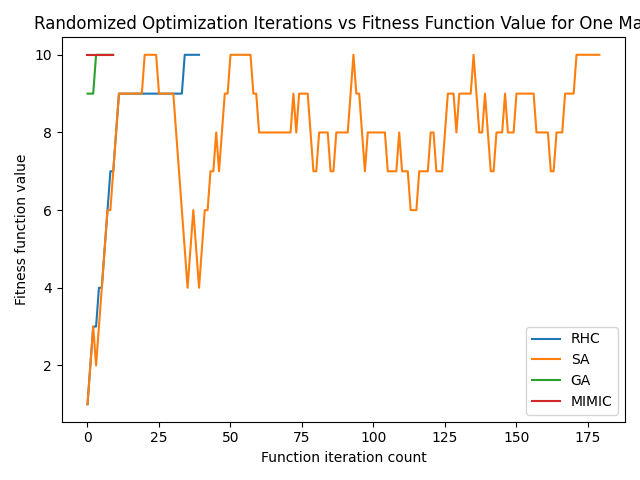
\includegraphics[width=.9\linewidth]{onemax1.png}
            \caption{One Max Iterations vs Function Value}\label{Fig:One Max Iterations vs Function Value}
        \end{minipage}\hfill
        \begin{minipage}{0.4\textwidth}
            \centering
            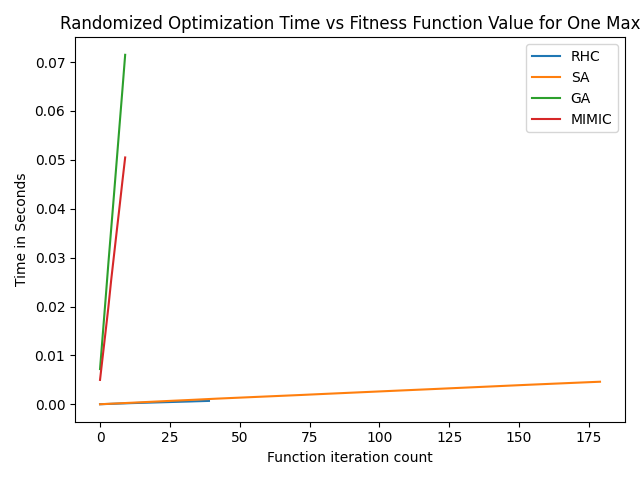
\includegraphics[width=.9\linewidth]{onemax2.png}
            \caption{One Max Iterations vs Time}\label{Fig:One Max Iterations vs Time}
        \end{minipage}
    \end{wrapfigure}
    \begin{wrapfigure}{c}{0.8\textwidth}
        \begin{center}
            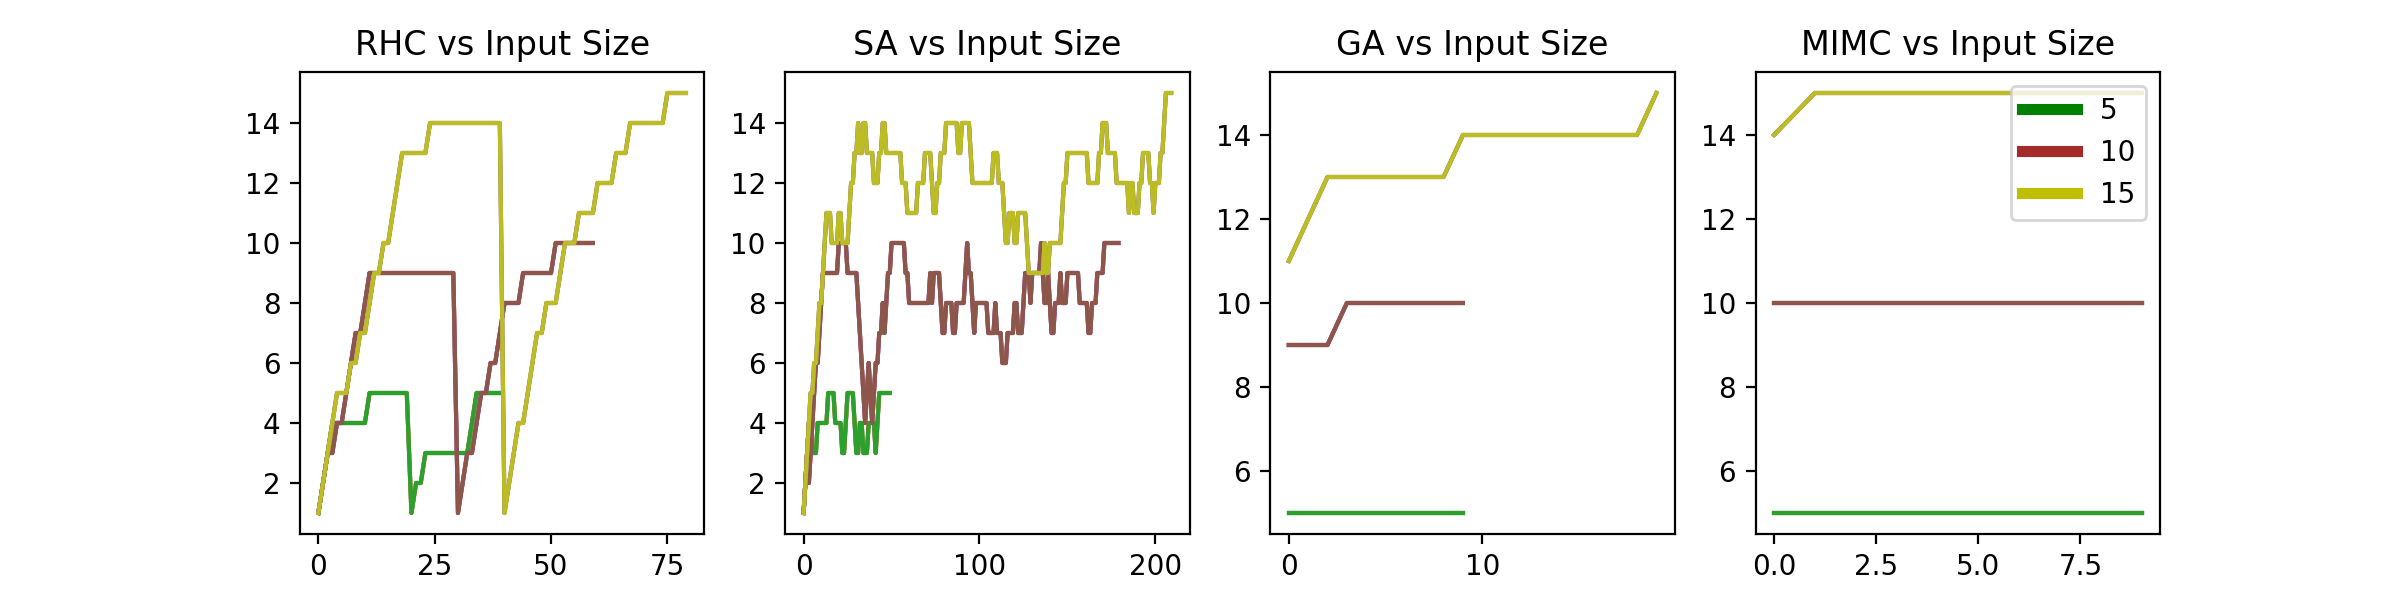
\includegraphics[width=1\linewidth]{onemaxinput.png}
            \caption{One Max Input Size vs Fitness Curve}\label{Fig:One Max Input Size vs Fitness Curve}
        \end{center}
    \end{wrapfigure}
    \begin{wrapfigure}{l}{0.4\textwidth}
        \begin{center}
            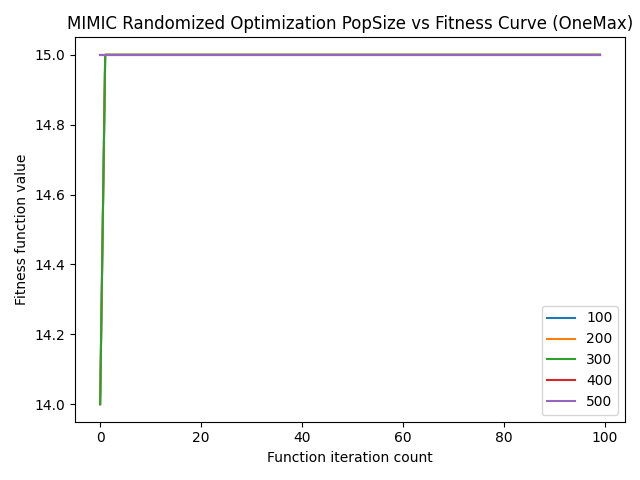
\includegraphics[width=1\linewidth]{onemaxmimic.png}
            \caption{One Max MIMIC PopSize vs Fitness Curve}\label{Fig:One Max MIMIC PopSize vs Fitness Curve}
        \end{center}
    \end{wrapfigure}
    Figures~\ref{Fig:One Max Iterations vs Function Value} and~\ref{Fig:One Max Iterations vs Time} illustrate how quickly MIMIC converged and that it took less wall clock time to do so than Genetic Algorithms
    (a similar class of algorithm.)
    As well as figure~\ref{Fig:One Max Input Size vs Fitness Curve}~shows us that comparatively MIMIC converges quickly
    with respect to input size.
    This result is most likely due to the fact that while MIMIC requires time to calculate probability density functions,
    by using this to improve its guess each time it saw the most dramatic improvement between iterations.
    By contrast Simulated Annealing took over 175 iterations to converge to the the correct value.
    The reason for this is due to the schedule of decay of SA. Since this problem has only one best value for any n
    dimensional input (a vector containing all 1's,) by considering worse values as potentially better (in order to
    to avoid local maxima).
    The same could be said for randomized hill climbing.
    Given that it will randomly restart in a different location it could potentially sabotage its own search for a maximum
    because the solution has only one max.
    The best performing class of algorithms were GA's and MIMIC for this problem, with MIMIC being a clear winner in terms
    of number of iterations required to find the optimal value.
    Because GAs/MIMIC are predisposed to favor well fitting values from previous generations to create a new generation
    of values this problem highlights this strength.
    Since there is only one max and by flipping one bit each time from a 0 to a 1 increases fitness, each algorithm would
    do successively better with each iteration.
    MIMIC did especially well because it could sample from a probability distribution of good values to create the next generation
    increasing the speed (in terms of iterations) of converging to the optimal value.
    It is worth noting however from a wall-clock time perspective, in general MIMIC performs worse than Genetic Algorithms
    because of the time required to recalculate $p^{\theta_i} (x)$ for the next generation as given by the definition of $p^{\theta_i} (x)$.\cite{Isbell97}

    \subsection{\problemtwo \hspace{0em}; highlights advantages of Simulated Annealing}
    The eight queens problem is a specific implementation of the n-queens optimization problem.\cite{Russel10} It poses
    an $n x n$ board like in chess where $n$ queens need to be placed such that a minimum number of queens could "attack"
    each other (diagonally, horizontally, or vertically.) So the space to search is a collection of vectors of 8 elements
    where each element is an integer between 0 and 7 and represents where the queen is on that column of the chess board.
    \begin{wrapfigure}{c}{0.8\textwidth}
        \begin{minipage}{0.4\textwidth}
            \centering
            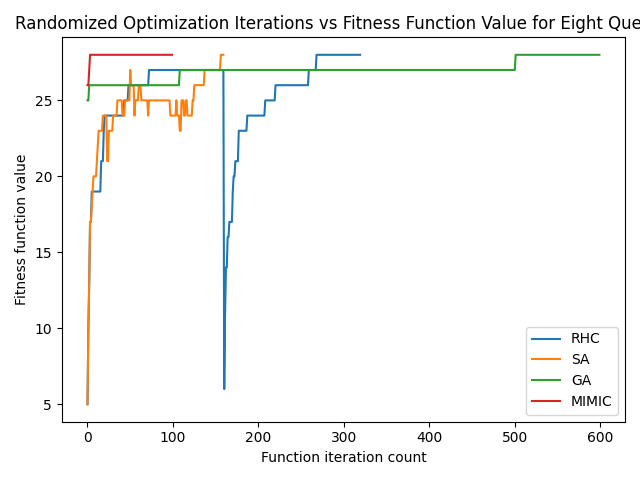
\includegraphics[width=0.9\linewidth]{eightqueens1.png}
            \caption{Eight Queens Iterations vs Fitness Function Value}\label{Fig:Eight Queens Iterations vs Fitness Function Value}
        \end{minipage}\hfill
        \begin{minipage}{0.4\textwidth}
            \centering
            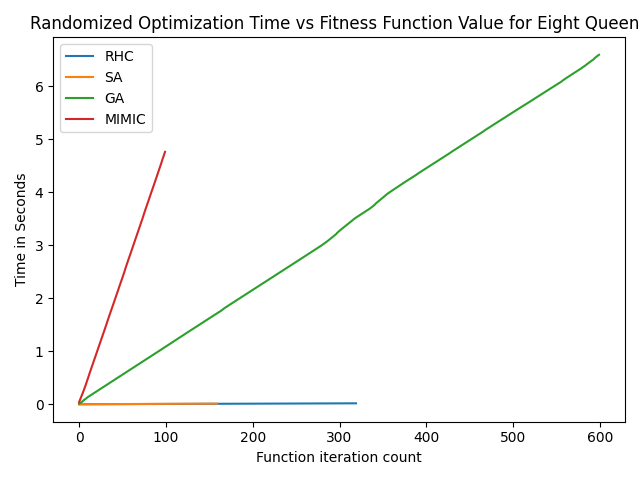
\includegraphics[width=0.9\linewidth]{eightqueens2.png}
            \caption{Eight Queens Iterations vs Time}\label{Fig:Eight Queens Iterations vs Time}
        \end{minipage}
    \end{wrapfigure}
    \begin{wrapfigure}{c}{0.4\textwidth}
        \begin{center}
            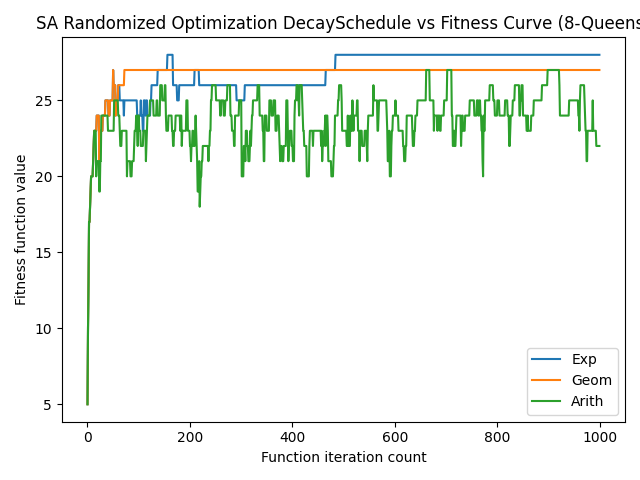
\includegraphics[width=1\linewidth]{eightqueensdecay.png}
            \caption{8-Queens SA DecaySchedule vs Fitness Curve}\label{Fig:8-Queens SA DecaySchedule vs Fitness Curve}
        \end{center}
    \end{wrapfigure}
    As illustrated below, this optimization problem favors the simulated annealing algorithm implementation approach I have chosen
    in terms of function iteration count required to achieve an optimal placement.
    The best values found for each algorithm were as follows:
    \begin{center}
        \begin{tabular}{| c | c | c |}
            \hline
            Algorithm & Parameters                                            & Value                 \\
            \hline
            \hline
            RHC       & Max Iterations, Max Attempts, Restarts                & 160, 160, 1           \\
            \hline
            SA        & Max Iterations, Max Attempts, Decay Schedule          & 160, 160, Exponential \\
            \hline
            GA        & Max Iterations, Max Attempts, Pop Size, Mutation Prob & 600,600,100,0.1       \\
            \hline
            MIMIC     & Max Iterations, Max Attempts, Pop Size, Keep \%       & 100,100,800,0.1       \\
            \hline
        \end{tabular}
    \end{center}
    The 8-Queens problem favors the Simulated Annealing algorithm I used (and somewhat the RHC algorithm as well) due to the nature of the problem.
    Because there are at maximum 92 solutions that are valid (derived from 12 fundamental solutions,)\cite{wikipedia_2020} and
    those maximal fitness values are dispersed throughout the space of all possible board states, algorithms like GA and
    MIMIC are at a disadvantage, because permuting random sections of a partially-fit vector do not necessarily equate to a
    strictly better fit vector.
    However in the case of SA and RHC which search for any maximal value through neighbor searching, these algorithms can directly
    compute an answer quickly often with an aggressive decay schedule since there are 92 best values each of which have the
    same fitness function value.
    In terms of wall clock time, Simulated Annealing did the best with a near zero wall clock time and only 160 function iterations to
    achieve the best result.
    While MIMIC did have a lower function iteration count required to get the best value, it used a population size of 800
    to achieve this and at a very steep cost in terms of computation time.
    Looking at figure 4, you can see that while Genetic Algorithms took the longest, MIMIC grew the fastest with respect to function
    iteration count, meaning that if we were to optimize an n-queens problem ($n > 8$), the lower iteration count would stop
    being a benefit in terms of wall-clock time quickly.

    \subsection{\problemthree \hspace{0em}; highlights advantages of Genetic Algorithms}
    The \problemthree is defined by mlrose's documentation in the following way:
    "The travelling salesperson problem (TSP) is a classic optimization problem where the goal is to determine the shortest tour of a collection of n 'cities' (i.e. nodes), starting and ending in the same city and visiting all of the other cities exactly once.
    In such a situation, a solution can be represented by a vector of n integers, each in the range 0 to n-1, specifying the order in which the cities should be visited."\cite{Hayes19}
    This problem is similar to the \problemtwo in that the vector represents an ordering of positions.
    In the \problemtwo they are board postions but in \problemthree they represent an order of cities to visit.
    Below is the table of optimal values for each function and the iteration and timing curves.
    \begin{center}
        \begin{tabular}{| c | c | c |}
            \hline
            Algorithm & Parameters                                            & Value                 \\
            \hline
            \hline
            RHC       & Max Iterations, Max Attempts, Restarts                & 40, 40, 0             \\
            \hline
            SA        & Max Iterations, Max Attempts, Decay Schedule          & 110, 110, Exponential \\
            \hline
            GA        & Max Iterations, Max Attempts, Pop Size, Mutation Prob & 100,100,100,0.1       \\
            \hline
            MIMIC     & Max Iterations, Max Attempts, Pop Size, Keep \%       & 100,100,200,0.1       \\
            \hline
        \end{tabular}
    \end{center}

    \begin{wrapfigure}{c}{0.8\textwidth}
        \begin{minipage}{0.4\textwidth}
            \centering
            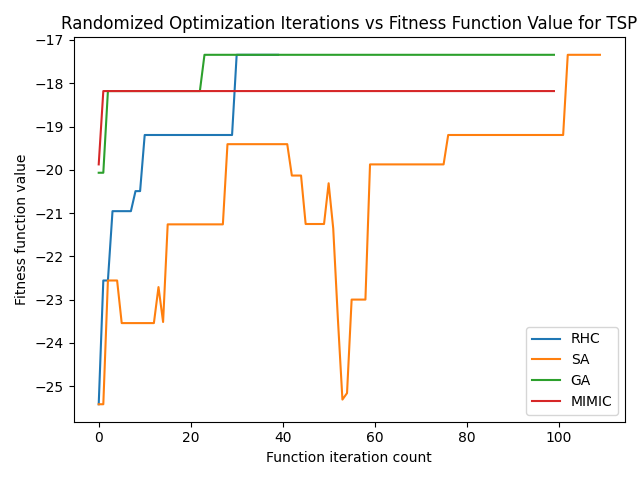
\includegraphics[width=0.9\linewidth]{tsp1.png}
            \caption{TSP Iterations vs Fitness Function Value}\label{Fig:TSP Iterations vs Fitness Function Value}
        \end{minipage}\hfill
        \begin{minipage}{0.4\textwidth}
            \centering
            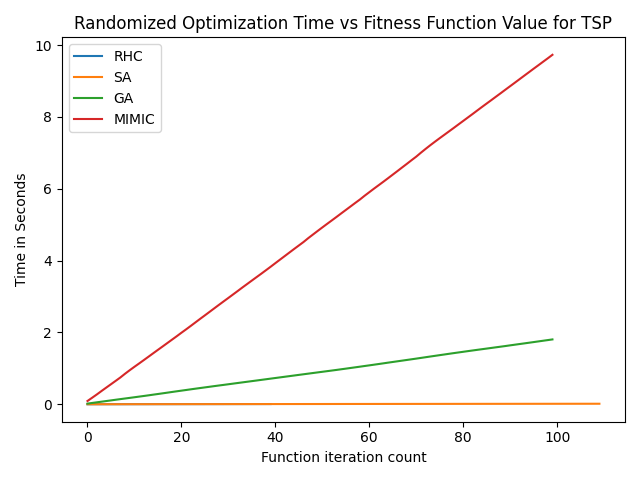
\includegraphics[width=0.9\linewidth]{tsp2.png}
            \caption{TSP Iterations vs Time}\label{Fig:TSP Iterations vs Time}
        \end{minipage}
    \end{wrapfigure}
    \begin{wrapfigure}{c}{0.4\textwidth}
        \begin{center}
            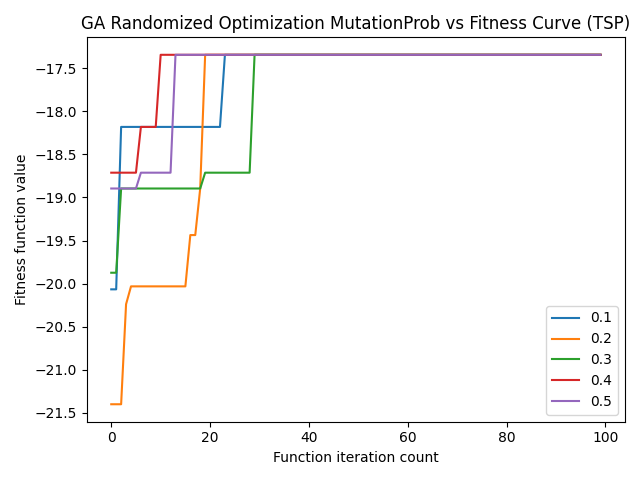
\includegraphics[width=1\linewidth]{tspmutprob.png}
            \caption{TSP GA MutationProb vs Fitness Curve}\label{Fig:TSP GA MutationProb vs Fitness Curve}
        \end{center}
    \end{wrapfigure}
    As you can see, the best all around algorithm in terms of speed and iteration count is Genetic Algorithms.
    While Simulated Annealing was faster in terms of wall clock time, Genetic algorithms got to the convergence value in
    a much shorter ($> 80$) number of iterations.
    Simulated Annealing and RHC would have the same advantages over GA and MIMIC in terms of their ability to search neighboring
    solutions for a max value easily as they did in 8-queens, the difference here is in the problem statement.
    Since the \problemthree is about minimizing the number of revisits to any point, it can be thought of as a constrained
    One Max problem (in that there is a best solution with the fewest number of revisits and there is only one global min.)
    In this way, the problem is like a combination of One Max and 8 queens.
    Given that, Genetic Algorithms ability to rapidly recombine better and better solutions allowed it to converge quickly
    to the correct value.
    The difference here is, whereas MIMIC is a variant of GA and in general performs better in the number of function iterations
    required to solve the same problem, in this instance MIMIC never converged to the globally minimal solution and even the
    sub optimal path ordering it proposed took 5x the amount of time as the nearest algorithm.


    \section{Neural Network Weight Optimization}
    In this section I will be applying the algorithms (with the exception of MIMIC) from above on my original assignment 1 dataset 1 (Classifying whether
    or not someone makes less than \textdollar50k in a year in America) and attempt to optimize a Neural Network's weights.
    The goal is to replace backpropagation as the method of NN training with RO\@.
    As was the case with the initial training I will be doing the following:
    \begin{itemize}
        \item Splitting the data into training and validation sets
        \item Optimizing for Jaccard Accuracy Score\cite{wikipedia_2021}
    \end{itemize}
    If you'll recall from the previous assigment, the NN did the worst out of all of the supervised learning algorithms from
    the previous section.
    This was due to the networks hidden layer construction and the fact that this problem did not lend itself well to any
    of the activation functions supplied to backpropagation as well as the fact that relative to the other learners, the
    best NN was subject to high bias given its underfitting.
    The best overall accuracy achieved was 75.14\% in total and that is what I targeted as an optimal value for the RO algorithms.
    I supplied the best overall hyperparameters from the previous assignment as arguments to mlrose's function for NN weight optimization
    to allow for a more direct comparison of results.
    Below is a table of the optimally tuned RO algorithms and their loss function values after training.

    \begin{center}
        \begin{tabular}{| c | c | c | c |}
            \hline
            Algorithm & Train/Test Accuracy & Loss Function Value & Param Values                 \\
            \hline
            \hline
            RHC       & 65.92\%/65.90\%     & 1.096               & Restarts=0                   \\
            \hline
            SA        & 65.90\%/65.90\%     & 1.096               & Schedule=ExpDecay            \\
            \hline
            GA        & 76.10\%/75.65\%     & 8.157               & PopSize=100 MutationProb=0.1 \\
            \hline
        \end{tabular}
    \end{center}
    Let's now look at the fitness curve and timing curve for these algorithms:
    As you can see from the fitness function curve, none of the three algorithms even change value during the optimization
    of the weights, suggesting that the initial guess remains the same for the entire training period.
    I did an experiment where I extend the max iterations out far beyond the graph's iteration count an there was no improvement.
    Disappointingly this makes it difficult to compare the performance of the various algorithms given that their values
    remained static regardless of parameter tuning.
    The only interesting thing to note was the amount of time Genetic Algorithms took relative to RHC and SA.
    It was significantly longer and increased linearly with iteration count whereas RHC and SA were more or less $O(c)$ in performance.
    This would seem to imply that each algorithm can do no better in terms of minimizing the loss function than its initial guess.
    The algorithm that did the best in terms of accuracy despite the fitness curve implying that it was entirely up to the first
    guess was Genetic Algorithms.
    It had a better overall accuracy on both training and testing sets than backpropagation despite having the highest value
    for a loss function.
    \begin{figure}
        \begin{minipage}{0.5\textwidth}
            \centering
            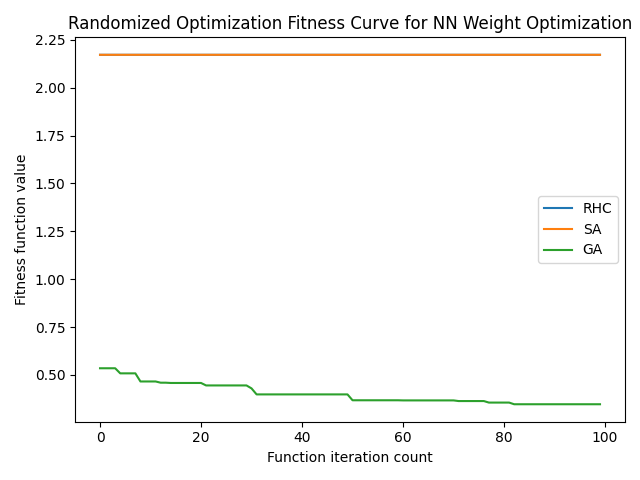
\includegraphics[width=0.9\linewidth]{nn1.png}
            \caption{NN Optimization Iterations vs Fitness Function Value}\label{Fig:NN Optimization Iterations vs Fitness Function Value}
        \end{minipage}\hfill
        \begin{minipage}{0.5\textwidth}
            \centering
            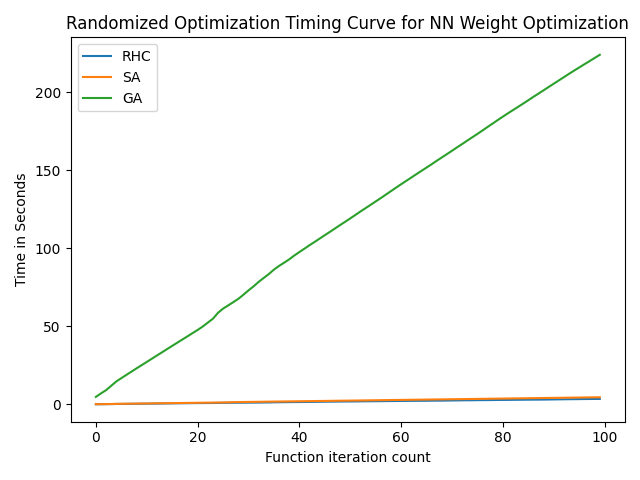
\includegraphics[width=0.9\linewidth]{nn2.png}
            \caption{NN Optimization Iterations vs Time}\label{Fig:NN Optimization Iterations vs Time}
        \end{minipage}
    \end{figure}
    After adjusting the learning rate to $1 x 10^{-5}$ and changing the \texttt{clip\_max} to 1, this still had no effect on the
    loss function and overall accuracy of the neural network.
    While it is near impossible to tell from the graphs, a closer look at the weights themselves shows small ($< 0.001$)
    changes in the fitness values for each function.
    RHC and SA while doing worse in terms of accuracy actually have a smaller loss function value, and therefore would likely
    generalize better over the unseen new data.
    GA while having a greater accuracy did so by training the network weights such that it always produced the guess for
    any new sample.
    Since the data is skewed (almost 75\% of one label) this guess ended up being more correct but would generalize worse
    as indicated by a worse overall loss function value.
    To improve this result I would need to further address/tune some of the following:
    \begin{itemize}
        \item Different activation functions
        \item Adjusting the learning rate
        \item Further adjusting hyper parameters of each RO algorithm
    \end{itemize}
    Below is a plot where I varied the Activation Functions for all of the RO algorithms during weight training.
    This shows for RHC and SA that the activation functions produced the same value for all iterations (despite being different.)
    This also shows for Genetic Algorithms that the Identity function reduced the loss function the most dramatically, while
    all of them improved.
    Genetic algorithms performed the best in terms of learning, and overall accuracy, but not in terms of time to train.
    \begin{figure}
        \begin{center}
            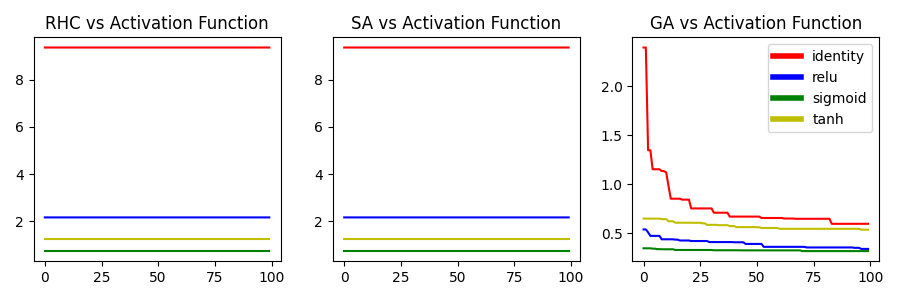
\includegraphics[width=1\linewidth]{nnactfunc.png}
            \caption{NN Activation Function vs Fitness Curve}\label{Fig:NN Activation Function vs Fitness Curve}
        \end{center}
    \end{figure}
    \pagebreak
    \bibliography{assignment2}
    \bibliographystyle{plain}
\end{document}